\documentclass[10pt, oneside]{article} 
\usepackage{amsmath, amsthm, amssymb, calrsfs, wasysym, verbatim, bbm, color, graphics, geometry}
\usepackage{polski}
\usepackage[utf8]{inputenc}
\usepackage[cache=false]{minted}
\usepackage{algorithm}
\usepackage{algorithmicx}
\usepackage[noend]{algpseudocode}
\usepackage{url}
\usepackage{tikz}
\usepackage{pgfplots}
\usepackage{booktabs}

\usetikzlibrary{matrix,arrows,automata}

\geometry{tmargin=.75in, bmargin=.75in, lmargin=.75in, rmargin = .75in}  

\theoremstyle{remark}
\newtheorem*{example}{Przykład}


% Cormen's cost analysis
\newcommand{\TITLE}[1]{\item[#1]}
\renewcommand{\algorithmiccomment}[1]{$/\!/$ \parbox[t]{4.5cm}{\raggedright #1}}
% ugly hack for for/while
\newbox\fixbox
\renewcommand{\algorithmicdo}{\setbox\fixbox\hbox{\ {} }\hskip-\wd\fixbox}
% end of hack
\newcommand{\algcost}[2]{\strut\hfill\makebox[1.5cm][l]{#1}\makebox[4cm][l]{#2}}



\title{Sieci neuronowe -- notatki do kursu}
\author{mgr. inż Dominik Filipiak}
\date{Rok akademicki 2019/2020}

\begin{document}

\maketitle
\tableofcontents

\vspace{.25in}

Dokument ten jest pomocą dla prowadzącego i nie zastępuje w żaden sposób podręcznika akademickiego.
W dużej części bazuje on na: M. Nielsen, \emph{Neural Networks and Deep Learning}\footnote{\url{http://neuralnetworksanddeeplearning.com}}, Determination Press, 2015.

\section{Wprowadzenie do sieci neuronowych}
\subsection{Wielowarstwowy perceptron}

Zdefiniujmy \textbf{perceptron}, matematyczną reprezentację neuronu, który dla trzech binarnych wagi $x_1, x_2, x_3$, gdzie każda z nich to 0 lub 1, zwraca binarne wyjście (czyli również 0 lub 1).
\begin{figure}[htpb]
	\centering
	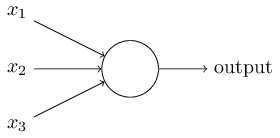
\includegraphics[width=.3\linewidth]{figures/tikz0}
	\caption{Perceptron z trzema binarnymi wejściami. Źródło: Nielsen (2015)}
\end{figure}
Możemy wprowadzić wagi $w_i$, które określą znaczenie każdego z wejść.
Jego wyjście będzie teraz równe ważonej sumie $\sum_j w_j x_j$.
W ogólności możemy to zapisać jako:
\begin{eqnarray}
  \mbox{output} & = & \left\{ \begin{array}{ll}
      0 & \mbox{if } \sum_j w_j x_j \leq \mbox{ threshold} \\
      1 & \mbox{if } \sum_j w_j x_j > \mbox{ threshold}
      \end{array} \right.
\end{eqnarray}

\begin{example}
Rozważmy problem decyzyjny -- czy wybrać się na festiwal?
Załóżmy, że zadecydują o tym trzy czynniki:
\begin{itemize}
	\item Czy pogoda jest dobra?
	\item Czy mój chłopak/dziewczyna pójdzie ze mną?
	\item Czy da się tam dojechać komunikacją miejską?
\end{itemize}
Oznaczymy odpowiedzi na te pytania. Niech $x_1 = 1$ jeżeli pogoda jest dobra, $x_1 = 0$ w przeciwnym razie.
Podobnie postąpimy z kolejnymi pytaniami.
Jeżeli bardzo chcemy iść na festiwal (więc możemy iść sami i zrezygnować z wygód komunikacji), ale nie znosimy złej pogody, to możemy to oznaczyć jako $w_1=6$, $w_2=2$, $w_3=2$.
Jeżeli ustawimy próg w sieci równy 5, to faktycznie odzwierciedli to nasze przekonania -- partner/partnerka oraz komunikacja miejska nie mają wpływu na wynik, ma go tylko pogoda.
Gdybyśmy natomiast zmniejszyli próg do 3, byłby to model, który reprezentowałby większą skłonność do wyjścia na festiwal.
\end{example}

Uprośćmy teraz nieco notację, a dokładniej warunek $\sum_j w_j x_j > \mbox{threshold}$.
Najpierw zapiszmy $\sum_j w_j x_j$ jako iloczyn skalarny $w \cdot x \equiv \sum_j w_j x_j$.
Próg (threshold) zastąpimy przez $b$ (ang. \emph{bias}), co fachowo nazywamy parametrem obciążenia transformacji afinicznej, gdzie $b \equiv -\mbox{threshold}$.

\begin{figure}[htpb]
	\centering
	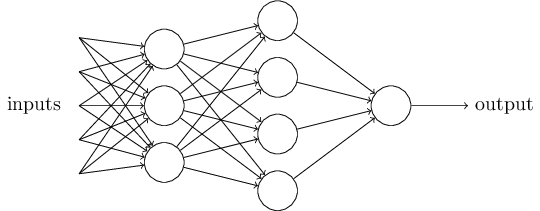
\includegraphics[width=.5\linewidth]{figures/tikz1}
	\caption{Prosta sieć. Źródło: Nielsen (2015)}
\end{figure}

\begin{eqnarray}
  \mbox{output} = \left\{ 
    \begin{array}{ll} 
      0 & \mbox{if } w\cdot x + b \leq 0 \\
      1 & \mbox{if } w\cdot x + b > 0
    \end{array}
  \right.
\end{eqnarray}



\subsection{Funkcja sigmoidalana}

W ogólności chcielibyśmy, żeby mała zmiana wag odpowiadała małej zmianie na wyjściu sieci.
W naszym przypadku mała zmiana potrafi jednak wszystko obrócić do góry nogami, tj. zamienić 0 na wyjściu w 1.
Modyfikacja wag jest więc problemem -- możemy sobie z nim poradzić wprowadzając nowy rodzaj neuronu, \textbf{funkcję sigmoidalną}.
\begin{figure}[htpb]
	\centering
	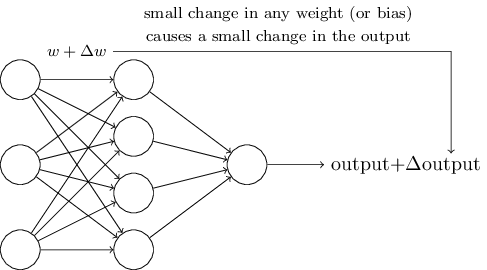
\includegraphics[width=.5\linewidth]{figures/tikz8}
	\caption{Prosta sieć. Źródło: Nielsen (2015)}
\end{figure}
Podobnie jak w perceptronie, taka funkcja ma ileś wejść -- tym razem jednak nie będą one w przedziale $[0, 1]$ (zamiast tylko 0 i 1) -- na przykład 0,638.
Zostawiamy również wagi oraz obciążenie.
Wyjście, podobnie jak wejście, znajduje się w zbiorze $[0, 1]$.
Określamy je jako $\sigma(w \cdot x+b)$, gdzie $\sigma$ definiujemy następująco:
\begin{eqnarray} 
  \sigma(z) \equiv \frac{1}{1+e^{-z}}.
\end{eqnarray}
Podstawiając dosłownie:
\begin{eqnarray} 
  \frac{1}{1+e^{\left(-\sum_j w_j x_j-b\right)}}.
\end{eqnarray}
Zauważmy, że jeżeli $z\equiv w \cdot x + b$ jest pewną dużą liczbą, to $e^{-z} \approx 0$ i tym samym $\sigma(z) \approx 1$.
Jeżeli natomiast $z$ jest \emph{bardzo} ujemną wartością, to $e^{-z} \rightarrow \infty$, dzięki czemu $\sigma(z) \approx 0$ -- patrz rys. \ref{fig:sigmoid} oraz \ref{fig:step}.
\begin{figure}[htpb]
	\centering
	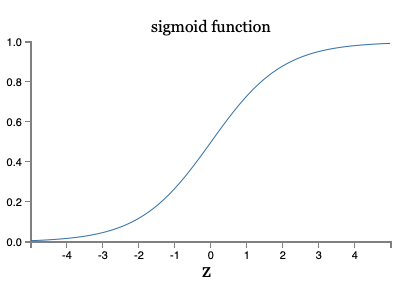
\includegraphics[width=.4\linewidth]{figures/sigmoid}
	\caption{Sigmoidalna funkcja aktywacji. Źródło: Nielsen (2015)}
	\label{fig:sigmoid}
\end{figure}
\begin{figure}[htpb]
	\centering
	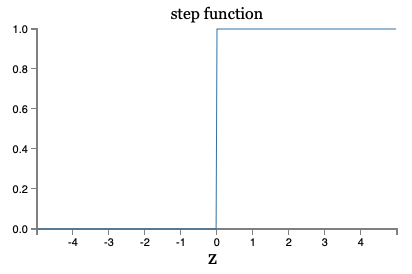
\includegraphics[width=.4\linewidth]{figures/step}
	\caption{Skokowa funkcja aktywacji. Źródło: Nielsen (2015)}
	\label{fig:step}
\end{figure}

Zastępując skokową funkcję przez funkcję sigmoidalną, uzyskujemy pewną matematyczną właśność.
Sigmoida jest funkcją gładką, tj. jest ona różniczkowalna nieskończenie wiele razy na swoim przedziale.
Gładkość implikuje też inne właściwości -- małe zmiany $\Delta w_j$ oraz $\Delta b$ powinny skutkować niewielką zmianą na wyjściu, co można aproksymować w następujący sposób:
\begin{eqnarray} 
  \Delta \mbox{output} \approx \sum_j \frac{\partial \, \mbox{output}}{\partial w_j}
  \Delta w_j + \frac{\partial \, \mbox{output}}{\partial b} \Delta b,
\end{eqnarray}

W ogólności funkcję $f$ postaci $f(w \cdot x + b)$ będziemy nazywać \textbf{funkcją aktywacji}.
Sieci wykorzystujące sigmoidalną funkcję aktywacji nazywane są czasami \textbf{wielowarstwowymi perceptronami} (ang. \emph{MLP}).



\subsection{Architektura sieci neuronowej}
Sieć neuronowa składa się, w ogólności, z trzech rodzajów warstw: \textbf{wejściowej}, \textbf{ukrytych}, oraz \textbf{wyjściowej}.
\begin{figure}[htpb]
	\centering
	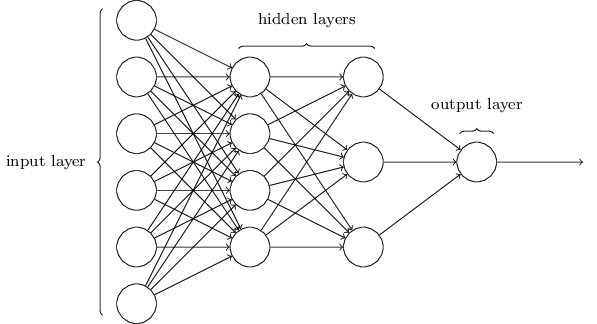
\includegraphics[width=.5\linewidth]{figures/tikz11}
	\caption{Architektura sieci. Źródło: Nielsen (2015)}
\end{figure}
Załóżmy, że chcemy klasyfikować obrazy przedstawiające cyfry zapisane odręcznie o rozmiarze $28 \times 28$ pikseli w skali szarości.
Ponieważ do reprezentacji każdego z nich z łącznie 764 pikseli w skali szarości potrzebujemy tylko jednej liczby (oznaczającej intensywność czerni), będziemy potrzebowali tylu neuronów na wejściu.
Zabawa zaczyna się przy dobieraniu liczby warstw ukrytych, a także ilości neuronów w każdej z nich.
W problemie klasyfikacji możemy dobrać liczbę neuronów na wyjściu tak, żeby reprezentowała liczbę klas -- ponieważ jest 10 cyfr, tylko neuronów będzie miała nasza sieć w warstwie wyjściowej.

\begin{figure}[htpb]
	\centering
	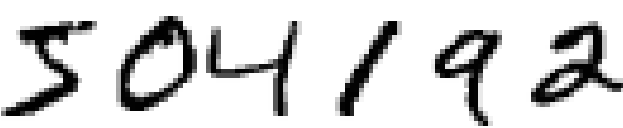
\includegraphics[width=.5\linewidth]{figures/digits}
	\caption{Cyfry zapisane odręcznie. Źródło: MNIST, Nielsen (2015)}
\end{figure}
\begin{figure}[htpb]
	\centering
	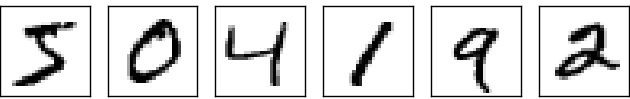
\includegraphics[width=.5\linewidth]{figures/digits_separate}
	\caption{Cyfry zapisane odręcznie po segmentacji. Źródło: MNIST, Nielsen (2015)}
\end{figure}
\begin{figure}[htpb]
	\centering
	
\includegraphics[width=.1\linewidth]{figures/mnist_first_digit}
	\caption{Pierwsza cyfra. Źródło: MNIST, Nielsen (2015)}
\end{figure}
\begin{figure}[!htpb]
	\centering
	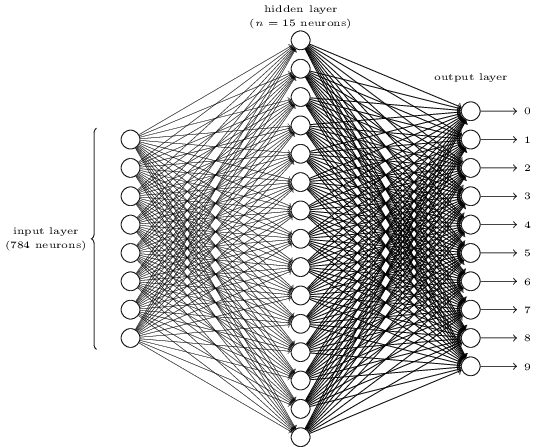
\includegraphics[width=.5\linewidth]{figures/tikz12}
	\caption{Architektura sieci. Źródło: Nielsen (2015)}
\end{figure}



\subsection{Błąd średniokwadratowy jako Funkcja kosztu}
Aby rozwiązać problem rozpoznawania odręcznie zapisanych cyfr, wprowadźmy najpierw kilka oznaczeń.
Niech $x$ to będzie nasze wejście, tym razem wektor o 784 wymiarach.
Wyjście oznaczymy przez $y=y(x)$, gdzie np. $y(x) = (0, 0, 0, 0, 0, 0, 1, 0, 0, 0)^T$ oznacza cyfrę 6.
Wprowadźmy teraz \textbf{funkcję kosztu}:
\begin{eqnarray}  C(w,b) \equiv
  \frac{1}{2n} \sum_x \| y(x) - a\|^2.
\end{eqnarray}
We wzorze tym $a$ oznacza wektor wyjść z naszej sieci dla $x$, natomiast $n$ oznacza liczbę rozpatrywanych przypadków testowych dla sieci (tj. liczbę cyfr, na których będziemy ją uczyć).
Ta funkcja jest nazywana często \textbf{błędem średniokwadratowym} (ang. \emph{MSE}).
Jej podstawowa własność to nieujemność.
Warto zauważyć, że jeżeli $y(x)$ jest podobne do $a$, to koszt powinien być blisko zera.
Tym samym określiliśmy \textbf{kryterium optymalizacyjne} naszego algorytmu do trenowania sieci neuronowej -- chcemy, aby zminimalizować koszt $C(w, b)$.
\begin{figure}[!htpb]
	\centering
	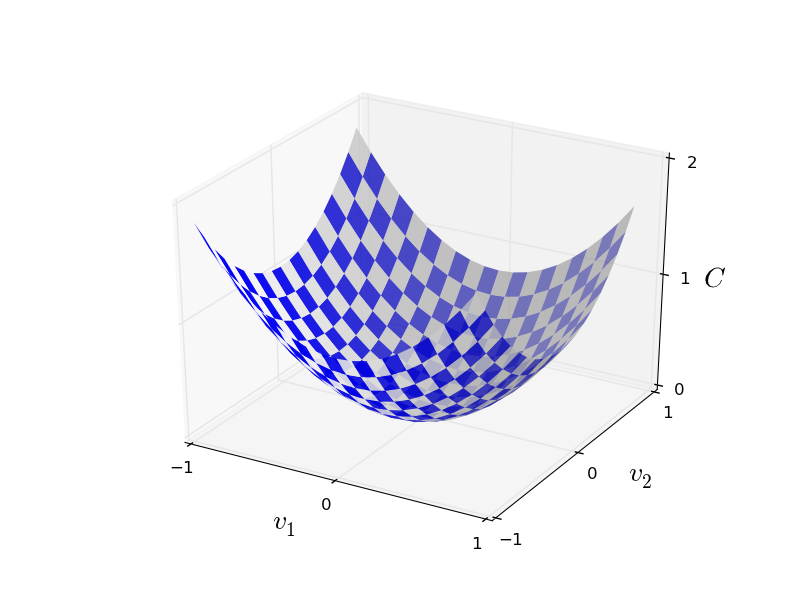
\includegraphics[width=.7\linewidth]{figures/valley}
	\caption{Wizualizacja wartości funkcji kosztu dla dwóch wymiarów. Źródło: Nielsen (2015)}
\end{figure}


\subsection{Spadek gradientu}

Wyznaczenie \textbf{globalnego minimum} dla funkcji kosztu w sposób analityczny jest możliwe dla funkcji niewielu zmiennych.
Dla funkcji wielu zmiennych jest to zadanie bardzo trudne.
Możemy się jednak posłużyć prostą heurystyką w poszukiwaniu lokalnego minimum, które często okazuje się być całkiem niezłe.
Wiedząc, że
\begin{eqnarray} 
  \Delta C \approx \frac{\partial C}{\partial v_1} \Delta v_1 +
  \frac{\partial C}{\partial v_2} \Delta v_2
\end{eqnarray}
oznaczmy $\Delta v \equiv (\Delta v_1, \Delta v_2)^T$.
Będziemy szukać takich $v$, które sprawią, że $\Delta C$ jest ujemne.
Następnie oznaczmy \textbf{gradient} jako $\nabla C$:
\begin{eqnarray} 
  \nabla C \equiv \left( \frac{\partial C}{\partial v_1}, 
  \frac{\partial C}{\partial v_2} \right)^T.
\end{eqnarray}
Tym samym możemy zapisać wszystko jako:
\begin{eqnarray} 
  \Delta C \approx \nabla C \cdot \Delta v.
\end{eqnarray}
Załóżmy teraz, że:
\begin{equation} 
  \Delta v = -\eta \nabla C,
  \label{eq:delta_v}
\end{equation}
gdzie $\eta$ to pewna wartość (zazwyczaj niewielka, np. 0,001) określająca \textbf{szybkość uczenia się}.
Wiemy, że $\Delta C \approx -\eta \nabla C \cdot \nabla C = -\eta \|\nabla C\|^2$. 
Ponadto, $\| \nabla C \|^2 \geq 0$, co gwarantuje, że $\Delta C \leq 0$ -- a taka własność jest bardzo oczekiwana w naszym problemie.
Tym samym jeżeli będziemy korzystać z równania \ref{eq:delta_v} do obliczenia $\Delta v$, to będziemy przesuwać naszą wirtualną piłkę z $v$ do $v'$ w następujący sposób:
\begin{eqnarray}
  v \rightarrow v' = v -\eta \nabla C.
\end{eqnarray}
\begin{figure}[!htpb]
	\centering
	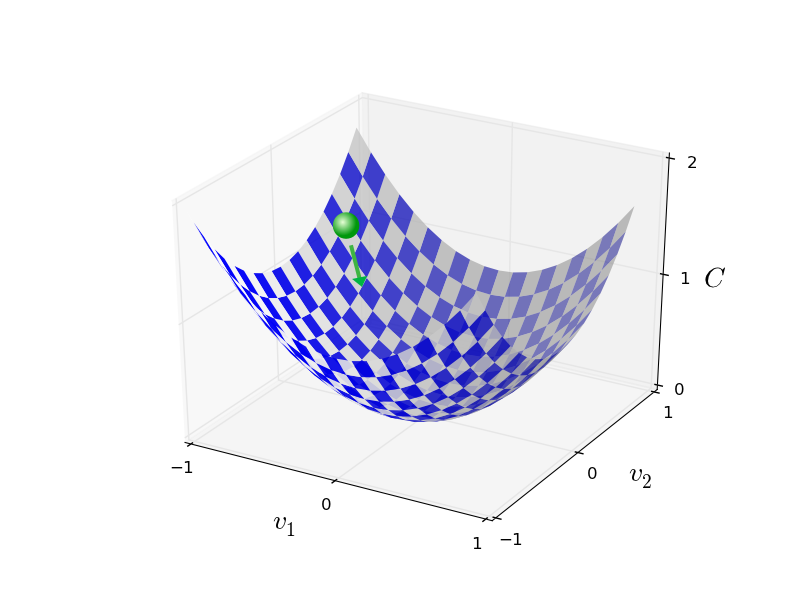
\includegraphics[width=.7\linewidth]{figures/valley_with_ball}
	\caption{Wizualizacja wartości funkcji kosztu dla dwóch wymiarów -- ilustracja spadku gradientu. Źródło: Nielsen (2015)}
\end{figure}


Dla funkcji wielu zmiennych wszystko działa tak samo, tj. dla $\Delta v = (\Delta v_1, \ldots, \Delta v_m)^T$ mamy:
\begin{eqnarray} 
  \Delta C \approx \nabla C \cdot \Delta v,
\end{eqnarray}
a gradient definiujemy w sposób następujący:
\begin{eqnarray}
  \nabla C \equiv \left(\frac{\partial C}{\partial v_1}, \ldots, 
  \frac{\partial C}{\partial v_m}\right)^T.
\end{eqnarray}
Z taką definicją dojdziemy do tych samych wniosków:
\begin{eqnarray}
  \Delta v = -\eta \nabla C,
\end{eqnarray}
co pozwala wyprowadzić regułę \textbf{spadku gradientu}:
\begin{eqnarray}
  v \rightarrow v' = v-\eta \nabla C.
\end{eqnarray}

Nie ma żadnych przeszkód do zastosowania tego algorytmu dla naszej sieci:
\begin{eqnarray}
  w_k & \rightarrow & w_k' = w_k-\eta \frac{\partial C}{\partial w_k} \\
  b_l & \rightarrow & b_l' = b_l-\eta \frac{\partial C}{\partial b_l}.
\end{eqnarray}


\subsection{Stochastyczny spadek gradientu}

\begin{eqnarray}
  \frac{\sum_{j=1}^m \nabla C_{X_{j}}}{m} \approx \frac{\sum_x \nabla C_x}{n} = \nabla C,
\end{eqnarray}

\begin{eqnarray}
  \nabla C \approx \frac{1}{m} \sum_{j=1}^m \nabla C_{X_{j}},
\end{eqnarray}

\begin{eqnarray} 
  w_k & \rightarrow & w_k' = w_k-\frac{\eta}{m}
  \sum_j \frac{\partial C_{X_j}}{\partial w_k} \\
  b_l & \rightarrow & b_l' = b_l-\frac{\eta}{m}
  \sum_j \frac{\partial C_{X_j}}{\partial b_l},
\end{eqnarray}

\subsection{Implementacja}

\begin{minted}{bash}
git clone https://github.com/mnielsen/neural-networks-and-deep-learning.git
\end{minted}


\end{document}